%% ==============================================================================
%%
%%  Document settings and macro definitions
%%
%% ==============================================================================

\documentclass[a4paper,10pt,bibtotoc]{scrartcl}
\usepackage{a4wide}
\usepackage{usg}
\usepackage{draftcopy}
\usepackage{upgreek}
\usepackage{jsonparse, booktabs}
%\usepackage[landscape]{geometry}
\usepackage{pdflscape}

\newcommand\sumline[2]{%
  \hbox to \linewidth{%
    \strut
    \parbox[t]{.85\linewidth}{\strut #1\strut}\hss
    \parbox[t]{.15\linewidth}{\raggedleft\strut #2\strut}%
  }
}



%% Do NOT remove: required to extract SVN information
\svnInfo $Id$

%% Adjust page footer
\fancyfoot[LE,LO]{LOFAR2-DDD-001: Transient Buffer Time-Series Data}
\fancyfoot[RE,RO]{\textsc{lofar} Project}

%% ==============================================================================
%%
%%  Document
%%
%% ==============================================================================

\begin{document}

\title{LOFAR Data Description Document:\\ Transient Buffer Time-Series Data\\
  {\normalsize Document ID: LOFAR2-DDD-001} \\
  {\normalsize Version 0.03.00} \\
   {\normalsize Persistent DOI: XXXXXX} \\
\author{ \parbox{\linewidth}{\centering S.~ter~Veen,  K. Mulrey, H.~Holties} }
\date{\small{Compile Date: \today}} 
}

\maketitle

\section{Table of contents}
\tableofcontents

\listoffigures

\listoftables

\clearpage

%% ______________________________________________________________________________
%%                                                                  Change record




\input common_tables/version_numbering




\clearpage

%%_______________________________________________________________________________
%%                                                                   Introduction

\section{Introduction}
\label{sec:introduction}

\begin{comment}
StV: acknowledge original authors?
\end{comment}

\subsection{Purpose and scope}
\label{sec:purpose and scope}

This data product definition document (DDD) describes the internal structure
of and the interface to the LOFAR time series data as generated by the Transient Buffers (TBufs). Time series data -- i.e. the digitised voltage output, as received by the individual LOFAR dipoles -- represent the primary input data to the cosmic ray and lightning analysis pipeline(s) and are the most basic form in which the received radio signals are present within the LOFAR
system. In LOFAR 1.0 these were referred to as the Transient Buffer Boards (TBBs); with the LOFAR 2.0 upgrade, the naming of this functionality changed to Transient Buffer (TBuf) as they do not have their own separate board. This document therefore serves as reference for the implementation of tools that read and write the TBuf data.

\subsubsection{Distinguishing LOFAR 2.0 data from older data}
To distinguish between the two file formats for the original LOFAR and the LOFAR 2.0 upgrade (executed in 2026), you can either check the \texttt{TELESCOPE\_VERSION} keyword or the \texttt{DOC\_NAME} in the header. For LOFAR 1.0 (TBB format) the \texttt{TELESCOPE\_VERSION} is not present. For LOFAR 2.0 (TBuf) the version is present with a  2.0 (or higher). The \texttt{DOC\_NAME} for LOFAR 1.0 data is \texttt{LOFAR-USG-ICD-001}. For LOFAR 2.0 data it is \texttt{LOFAR2-DDD-001}. Please also check the right \texttt{DOC\_VERSION} for your data files and software. %, see \ref{sec:tools}.



\subsection{Applicable Documents}
\input common_tables/applicable_to_all_documents



\begin{center}
  %% Table head
  \tablefirsthead{
    \hline
    \textsc{Reference} & \textsc{Title} & \textsc{Description} \\
    \hline
  }
  \tablehead{
    \multicolumn{3}{r}{\small \textbf{Applicable documents}
      \textsl{continued from previous page}} \\
    \hline
    \textsc{Reference} & \textsc{Title} & \textsc{Description} \\
    \hline
  }
  %% Table tail
  \tabletail{
    \hline
    \multicolumn{3}{r}{\small\sl continued on next page} \\
  }
  \tablelasttail{\hline}
  %% Table contents
  \bottomcaption[List of documents that apply to to this document]{
    List of documents that apply to this Documents.
  \label{tab:applicable list specific}}
  \begin{supertabular}{lp{5.8cm}p{7cm}}
    \shrinkheight{-4.5em}
    \texttt{ICD-001} \cite{lofar.icd.001} & TBB Timeseries-Data & Previous definition of the Transient Buffer Timeseries Dataformat as used by the previous LOFAR system (2009-2022). This document is based on that document. \\
    \hline
  \end{supertabular}
\end{center}


\subsection{Reference applications}
This document serves as reference for the
implementation of tools that read and write the TBuf data. A non-extensive list is provided here.

\begin{comment}
Update software list and provide links to applications (references, source code repository).
\end{comment}

\begin{center}
  %% Table head
  \tablefirsthead{
    \hline
    \textsc{Name} & \textsc{Title} & \textsc{Purpose} \\
    \hline
  }
  \tablehead{
    \multicolumn{3}{r}{\small \textbf{Applicable documents}
      \textsl{continued from previous page}} \\
    \hline
    \textsc{Reference} & \textsc{Title} & \textsc{Description} \\
    \hline
  }
  %% Table tail
  \tabletail{
    \hline
    \multicolumn{3}{r}{\small\sl continued on next page} \\
  }
  \tablelasttail{\hline}
  %% Table contents
  \bottomcaption[List of tools that read and/or write this data format]{
    List of tools that read and/or write this data format.
  \label{tab:applicable list}}
  \begin{supertabular}{lp{4.8cm}p{6cm}}
    \shrinkheight{-4.5em}
    \texttt{Cosmic Ray Pipeline} \cite{tools.2} & Cosmic Ray Pipeline & Pipeline to analyse cosmic ray data \\
    \texttt{Lightning mapper} \cite{tools.3} & Lightning imager &  3-D imager for lightning \\
    \hline
  \end{supertabular}
\end{center}
%% ______________________________________________________________________________
%%                                                              Section: Overview

\subsection{Overview}
\label{sec:overview}

This document is structured as follows: %
Section \ref{sec:structure} will describe fundamental overall
structure, including a statement of the primary data product format,
HDF5. These conventions will also include names, meaning, and physical
units that may be used to generate and interpret the data files. %
Section \ref{sec:detailed structure} will present a detailed
specification for the data, including a description of the structure
of a LOFAR TBB data naming conventions, units, physical quantities. %

%%_______________________________________________________________________________
%%                                                       Organisation of the data

\clearpage

\section{Organisation of the data}
\label{sec:structure}

\subsection{Conventions}

\input common_tables/types

\input common_tables/notation


\subsection{Data Structure}

A LOFAR TBuf Time-series data file will adhere to the following guidelines:\\

A LOFAR TBuf Times-series data file will be defined within the context
of the HDF5 file format.  A LOFAR TBuf Time-series HDF5 file structure
will comprise a primary group, a ``root group" in HDF5 nomenclature,
which may be considered equivalent to a primary header/data unit (HDU)
of a standard multi-extension FITS file.  This primary group will
consist only of header keywords (“attributes” in HDF5 nomenclature)
describing general properties of an observation, along with pointers
to contained subgroups.  Those subgroups will comprise an arbitrary
number of ``AntennaFieldGroups'' (see sec~\ref{sec:antenna field group}), where a
Antenna Field will contain data and meta-data produced by an
individual Antenna Field of an indvididual LOFAR station. Each antenna field group contains one or more ``Dipole Datasets``.

Figure~\ref{fig:TBB_highlevel} shows the basic organisation of the dataset within
the HDF5 format. The hierarchical structure essentially follows the
hierarchical structure of LOFAR itself, i.e. in a top-down approach
from array through stations through antenna fields down to individual dipoles. The grouping
of multiple antennas/dipoles within a station is mirrored by the
collection of dipole datasets into the antenna field groups.

\subsubsection{Overview of TBB Groups}

The structure of the file is subdivided into the following four HDF5 group levels:

\begin{enumerate}
\item \textbf{Root} (\verb|ROOT|). The root level of the file contains the
  majority of associated meta-data, describing the circumstances of
  the observation. These data attributes include observation time
  (start and end) and other important characteristics of the dataset. See
  section \ref{sec:root group} for further details.
\item \textbf{Trigger Group} (\verb|TRIGGER|). This
  group collects parameters generated by the trigger
  algorithm that requested the data. See section \ref{sec:trigger group} for further
  details.
\item \textbf{Antenna Field}(\verb|(ANTENNA_FIELD_{AAKKK}_{XXXN})|). This group serves as a
  common container for the separate sub-tables, which take up data from the dipoles and from the station calibration.
  The part first part between \verb|{...}| represents the station name and consists of 2
  characters (upper case) and three digits (e.g. 'CS001' or 'RS106'). The second part between \verb|{...}| represents the antenna field type and consists of 3 characters (upper case) and 0 or 1 digits (e.g. 'LBA' or 'HBA0'). 
  See section \ref{sec:antenna field group} for further details.
\item \textbf{Dipole Dataset} (\verb|DIPOLE_{SSSSS_TTTAAP}|). This group
  collects data on a per-dipole basis starting from the identifiers required for
  the unambiguous identification of an individual dipole within the full LOFAR
  network to the actual sampled wave-form of the EM-field at the position of
  each antenna feed. This group contains a dataset of the sampled raw voltages after analog-digital conversion.
  The part between \verb|{...}| represents the name of the dataset and is
  constructed from the \small \texttt{STATION\_NAME} (SSSSS), \verb|ANTENNA_TYPE| (TTT),\verb|ANTENNA_ID|
  (AA) and \verb|POLARIZATION| (P).
  See section \ref{sec:dipole dataset} for further details.
\end{enumerate}


%%_______________________________________________________________________________
%%                                                    Detailed Data Specification


\subsubsection{Hierarchical structure}
\label{sec:hierarchical structure}

\begin{figure}[htb]
  \centering
  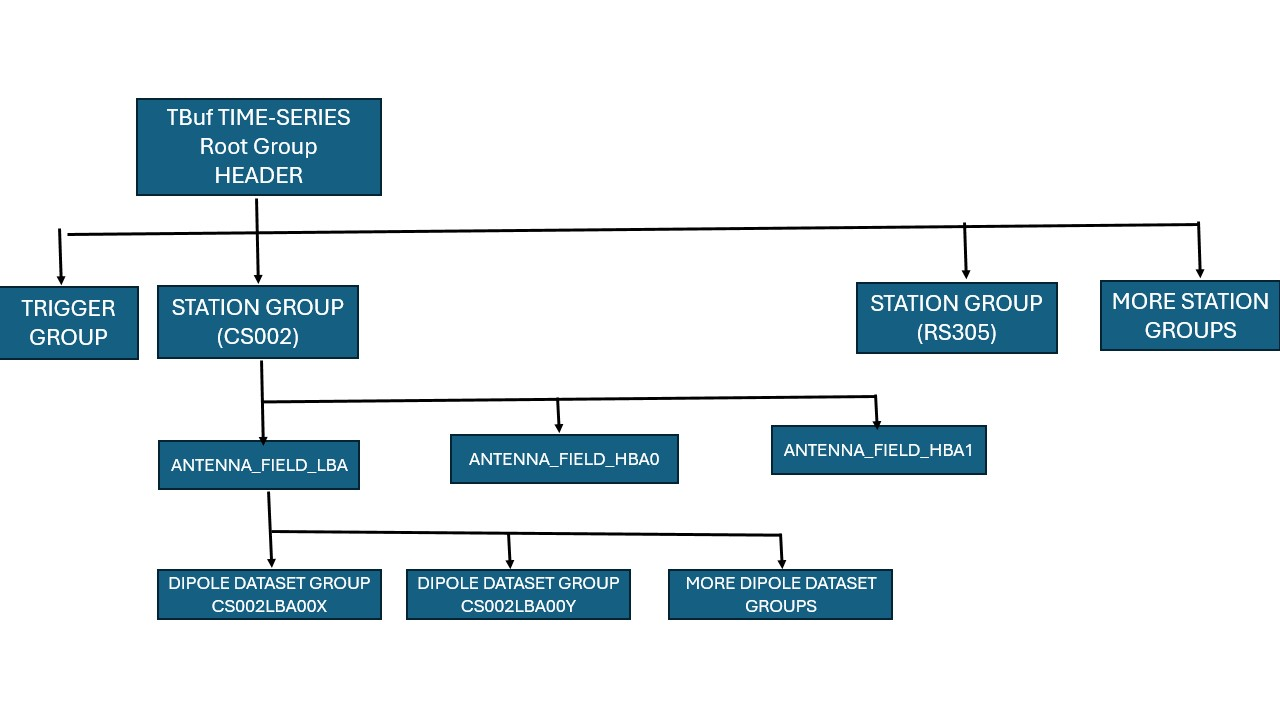
\includegraphics[width=\textwidth]{figures/TBuf_hierarchy.png}
  \caption[Hierarchical structure of a TBB times-series dataset.]{
    Hierarchical structure of a TBB times-series dataset; the
    internal organization of the data follows the hierarchical
    organization of the LOFAR system.}
  \label{fig:TBB_highlevel}
\end{figure}

{\small
\begin{verbatim}
/                                          ...  Root Group
|-- TRIGGER                                ...  Group
|-- ANTENNA_FIELD_XS123_XBA                ...  Group (Station name + antenna field (LBA, HBA, HBA0 or HBA1) )
|   |-- DIPOLE_{SSSSS_TTTAAP}                 ...  Dataset     [1D, short]
\end{verbatim}
}

This structure can be represented through HDF5 as a \textsc{posix}-style hierarchy:

Raw Voltage Mode:
\begin{verbatim}
/
/TRIGGER
/ANTENNA_FIELD_CS002_LBA/
/ANTENNA_FIELD_CS002_LBA/DIPOLE_CS002_LBA00X
/ANTENNA_FIELD_CS002_LBA/DIPOLE_CS002_LBA00Y
/ANTENNA_FIELD_CS002_LBA/DIPOLE_CS002_LBA01X
/ANTENNA_FIELD_CS002_LBA/DIPOLE_CS002_LBA01Y
/ANTENNA_FIELD_CS002_LBA/DIPOLE_CS002_LBA...
/ANTENNA_FIELD_CS002_HBA0
/ANTENNA_FIELD_CS002_HBA0/DIPOLE_CS002_HBA00X
/ANTENNA_FIELD_CS002_HBA0/DIPOLE_CS002_HBA00Y
/ANTENNA_FIELD_CS002_HBA0/DIPOLE_CS002_HBA01X
/ANTENNA_FIELD_CS002_HBA0/DIPOLE_CS002_HBA01Y
/ANTENNA_FIELD_CS002_HBA0/DIPOLE_CS002_HBA...
/ANTENNA_FIELD_CS002_HBA1
/ANTENNA_FIELD_CS002_HBA1/DIPOLE_CS002_HBA24X
/ANTENNA_FIELD_CS002_HBA1/DIPOLE_CS002_HBA24Y
/ANTENNA_FIELD_CS002_HBA1/DIPOLE_CS002_HBA25X
/ANTENNA_FIELD_CS002_HBA1/DIPOLE_CS002_HBA...
/ANTENNA_FIELD_RS305_LBA
/ANTENNA_FIELD_RS305_LBA/DIPOLE_RS305_LBA00X
/ANTENNA_FIELD_RS305_LBA/DIPOLE_RS305_LBA...
/ANTENNA_FIELD_RS305_HBA
/ANTENNA_FIELD_RS305_HBA/DIPOLE_RS305_HBA00X
/ANTENNA_FIELD_RS305_HBA/DIPOLE_RS305_HBA...
...
\end{verbatim}


%%______________________________________________________________________________
%%                                                   Detailed Data Specification

\clearpage

\section{Detailed Data Specification}
\label{sec:detailed structure}

\input common_tables/metadata_intro

\subsection{Naming}
The Transient Buffer Time-series files are named as follows:\\\,\\
\verb|L<ID>_D<date>T<time>Z_<stationname>_<fieldname>_R<part>_tbb.h5|\\\,\\
\verb|L<ID>_D<date>T<time>Z_<stationname>_<fieldname>_R<part>_tbb.raw|\\\,\\
Example:\\
\verb|L123456789_D20140123T134448.920Z_CS002_LBA_R000_tbb.h5|\\\,\\
\verb|L123456789_D20140123T134448.920Z_CS002_LBA_R000_tbb.raw|\\\,\\

In this 
\begin{itemize}
    \item L is an identifier for LOFAR. If used for different instrument, this can change.
    \item \verb|<ID>| is the subtaskID of the LOFAR TMSS process managing the data acquisition process. For this version that are the \verb|tbuf_dump| subtasks
    \item The \verb|<date>| and \verb|<time>| is either the requested start and end time of the data or the actual start and end time of the data. The actual start time of the data may be later then the requested start time and is annotated in the metadata of the file. The time is specified up till millisecond precision. The time is indicated in UTC, as also denoted by the Z.
    \item The \verb|<stationname>| is the name of the first station in the file.
    \item \verb|<fieldname>| is the name of the first antenna field in the file. One of (LBA, HBA, HBA0, HBA1, NNF). 
\end{itemize}
The lengths of the filename may vary because of the \verb|<ID>| and the \verb|<fieldname>|. The "h5" file contains the header information, as described in this document. The ".raw" file contains the actual data. This split is motivated to easily be able to read the "h5" file, for example to gather feedback. The end user should make sure both the "h5" and the "raw" file are copied over. 


\subsection{The Root Group}
\label{sec:root group}

The LOFAR file hierarchy begins with the top level \verb|`Root`| Group.  This is
the file entry point for the data, and the file node by which navigation of
the data is provided. The \texttt{Root} group will comprise a set of attributes
that describe the underlying file structure, observational metadata, the LOFAR
TBuf data, as well as providing hooks to all groups attached to the \texttt{Root} group.

This section will specify two sets of attributes that will appear in
the \texttt{Root} group: a set of \cla\ (CLA) that will be common to
all LOFAR science data products, and a set of attributes that are
specific to LOFAR TBB Time-series data.  Though these attributes will
all appear together in the \texttt{Root} attribute set, they are
separated in this document in order to demarcate those general LOFAR
attributes that are applicable across all data, and those attributes
that are TBB-specific.\\
In other words,

\begin{verse}
\verb|Root Attributes = Common LOFAR Attributes (CLA) + Supplemental TBB Root Attributes.|
\end{verse}

The \cla\ are the first attributes of any LOFAR file root group.

\subsubsection{\cla}
\label{sec:common lofar attributes}

This section will specify a set of attributes that will be common to
LOFAR science data products.  These ``common LOFAR metadata'' will
appear as attributes at the root level of all LOFAR data files.
\textit{All} LOFAR data products, including TBuf Time-series
\textit{inter alia,} will share a common set of metadata root-level
attributes.  These common LOFAR metadata are to be the first set of
attributes of any LOFAR file root group.

Table~\ref{tab:lofar common metadata} lists the {\cla} (CLA) which can
be found in LOFAR observation mode data types. These Attributes are required to be in the Root
Group; if a value is not available for an Attribute, a \verb|`NULL'|
will be used in its place. Special considerations for these keywords: \texttt{OBSERVATION\_ID} contains the subtask ID of the data acquisition specific for this trigger. Other \texttt{OBSERVATION...} keywords consider the data for this trigger/file, for example the \texttt{OBSERVATION\_START\_UTC} is the start of the data dump. The \texttt{OBSERVATION\_FREQUENCY...} keywords refer to the whole band for this filter, or for all filters used. For example the \texttt{110\_190 MHz} filter will provide a min,center,max frequency of 100, 150, 200 Mhz, respectively. \texttt{OBSERVATION\_NOF\_BITS\_PER\_SAMPLE} is 12 for TBuf data. \texttt{FILTER\_SELECTION} and \texttt{ANTENNA\_SET} are usually set to \texttt{NULL}. They are repeated at lower levels. They can be set to the actual value, if and only if a single value is used at lower level within this file, but this is not obligatory as pipelines should better rely on the value per dipole.

\begin{table}[tbp]
  \centering
  \begin{tabular}{|lrp{6cm}|}
    \hline
    \textsc{General LOFAR Group} & \textsc{Value} & \textsc{Description} \\
    \hline
    Root          & \verb|`Root'|    & Top-level LOFAR group type.\\
    \hline
    \hline
    \textsc{TBB Specific Groups} & \textsc{Value} & \textsc{Description} \\
    \hline
    
    Trigger group & \verb|`TriggerGroup'| &  Trigger data group. \\
    Antenna Field group & \verb|`AntennaFieldGroup'|  & Antenna Field data group. \\
    Dipole dataset & \verb|`DipoleDataset'| & Individual Dipole Dataset (Raw Voltage Mode). \\
    % Processing History group &\verb|`ProcessHist'| & This is a Processing History group. \\
    \hline
  \end{tabular}
  \caption{LOFAR TBB Time-series Group Types.}
  \label{tab:group types}
\end{table}


\input common_tables/lofar_common_metadata

\subsubsection{Additional TBuf Time-series Root Attributes}
\label{sec:additional root group attributes}

As explained at the beginning of Sec.~\ref{sec:root group} above, the
root group of a \textbf{TBuf Time-series data file} will contain a set
of attributes, which can be broken down into two subsets: 1) a set of
\cla\ (CLA) that will be common to all LOFAR science data products,
and 2) a set of attributes that are specific to LOFAR Time-series data
(see Table~\ref{tab:hdf5 root group}). With the {\cla} already listed
in section~\ref{sec:common lofar attributes} above, this section will
focus on the second subset of root group attributes, as they are
specific to a \textbf{TBuf Time-series data file}.

\begin{table}[htbp]
  \centering
  \begin{tabular}{|llp{9cm}|}
    \hline
    \textsc{Field/Keyword} & \textsc{Type} & \textsc{Description} \\
    \hline
    \hline
    %\verb|NOF_STATIONS| & \verb|unsigned| &  The number of station groups
    %available in the file.\\
    \verb|ANTENNA_FIELD_{AAKKK}_{XBAX}| & Group & Antenna field group collecting the data
    from an individual LOFAR station; It consists of the station name with 2
    characters (upper case) and three digits, followed by the antenna field name (LBA, HBA, HBA0, HBA1.\\
    \verb|TRIGGER| & Group & Group collecting the
    parameters associated with the trigger and the output
    parameters generated by it. \\
    \hline
  \end{tabular}
  \caption{Additional attributes and objects attached to the root
    group of a TBB time-series data file.}
  \label{tab:hdf5 root group}
\end{table}

\clearpage



%%_______________________________________________________________________________
%%                                                    Trigger Group 
\clearpage %% Needed for correct positioning the long trigger group table
           %% w.r.t. other tables.

\paragraph{Trigger Group}

\label{sec:trigger group}

The \verb|TRIGGER| group collects the parameters that caused the TBB to be frozen and the data to be collected. Table~\ref{tab:trigger group} shows the attributes within this group.




\begin{center}
  \tablefirsthead{%
    \hline
    \textsc{Field/Keyword} & \textsc{Type} & \textsc{Software} & \textsc{Description} \\
     && \textsc{Version} &\\
    \hline\hline
  }
  \tablehead{
    \multicolumn{4}{r}{\small\textsl{Table \ref{tab:trigger group}: continued from previous page}}\\
    \hline
    \textsc{Field/Keyword} & \textsc{Type} & \textsc{Software} & \textsc{Description} \\
     && \textsc{Version} &\\
    \hline\hline
  }
  \tabletail{
    \hline
    \multicolumn{4}{r}{\small\textsl{Table \ref{tab:trigger group}: continued on next page}}\\
  }
  \tablelasttail{
    \hline
  }
  \bottomcaption{Attributes attached to a TRIGGER group (TriggerGroup).}
  \begin{supertabular}{|lllp{5.25cm}|}
    \small \texttt{GROUPTYPE} & \verb|string| & DDD v1.0.0 & The value of the grouptype is \verb|`TriggerGroup'|.\\
    \small \texttt{TRIGGER\_TYPE} & \verb|string| & DDD v1.0.0 & Type of trigger. The default value is ``Unknown''.\\
    \small \texttt{TRIGGER\_SUBTYPE} & \verb|string| & DDD v1.0.0 & SubType of trigger. The default value is ``Unknown''.\\
    \small \texttt{TRIGGER\_VERSION} & \verb|string| & DDD v1.0.0 & Version of the trigger algorithm, following Semantic Versioning 2.0.0\footnote{www.semver.org}. The default value is 1.0.0. \\
    \small \texttt{TRIGGER\_ID} & \verb|string| & DDD v1.0.0 & Identifier to match with parameters from the detector/script that sent the trigger. \\
    \small \texttt{TIME} & \verb|unsigned| & DDD v1.0.0 & Unix Timestamp of the trigger in number of seconds since January 1, 1970, 00:00:00 UTC.\\
    \small \texttt{SAMPLE\_NUMBER} & \verb|unsigned| & DDD v1.0.0 & Subsecond timestamp of the trigger expressed as sample number inside the second marked by \verb|TIME|, assuming 5 ns samples. \\
    \small \textit{\texttt{ADDITIONAL\_INFO}} & \verb|string| & DDD v1.0.0 & Free form text field. \\
    \hline
  \end{supertabular}
  \label{tab:trigger group}
\end{center}

The type of trigger is given by the keyword \verb|TRIGGER_TYPE| and \verb|TRIGGER_SUBTYPE|. They contain keywords from Table~\ref{tab:trigger_types}.

\begin{table}[htb]
  \centering
  \begin{tabular}{|lp{9cm}|}
    \hline
    \textsc{Value of} \verb|TRIGGER_TYPE| & \textsc{Description} \\
    \hline
    \hline
    \verb|`Unknown'| & Unknown/unrecognised reason for data return. \\
    \verb|`LORA'| & Trigger to capture a cosmic ray. \verb|TRIGGER_SUBTYPE|  = 'LORA' when triggered from the LORA particle detector.\\
    \verb|`Lightning'| & Triggered in order to capture a lightning strike. \verb|TRIGGER_SUBTYPE| = 'blitzortung' or 'magnetic loop' \\
    \verb|`Manual'| & Manually triggered. \verb|TRIGGER_SUBTYPE| = 'User Portal' or 'test script'\\
   \hline
  \end{tabular}
  \caption{Values of TRIGGER\_TYPE.}
  \label{tab:trigger_types}
\end{table}

Additional keywords for trigger setup or other trigger values can be sent in \verb|ADDITIONAL_INFO|. These are highly detector dependent and will require their own description document. If they are described for a detector, please add the description document in the document list.

%%_______________________________________________________________________________
%%                                                    Antenna Field Group 

\subsection{The Antenna Field Group}
\label{sec:antenna field group}

With LOFAR 2.0, both the LBA and HBA antenna fields can be active at the same time and with different settings. Therefore the \texttt{StationGroup} from the original LOFAR TBB Time-series format is replaced by the \texttt{AntennaFieldGroup} 

Given the different modes for transient buffer observation, and that with LOFAR 2.0, both the LBA and HBA antenna fields can be active at the same time, a single LOFAR
antenna field is the natural choice for a first grouping of time-series
data from the individual dipoles; for that matter we consider the
\textbf{Antenna Field Group} (Table~\ref{tab:antenna field group}) as a basic module within
the data structure.\footnote{Though from initial perception the described
structure can be perceived as a table, the HDF5 internal data model is that
of a group; in order to stick as closely as possible to the libraries naming
conventions, we therefore use the name \textsl{group} instead of \textsl{table}.}
Creating a snapshot of multiple stations, or even the full LOFAR array, thus will
result in a set of antenna field groups -- which in turn might be collected into
another superstructure.

\newpage
\begin{landscape}
\begin{table}[htbp]
  \centering
  \begin{tabular}{|lllllp{5.5cm}|}
    \hline
    \textsc{Field/Keyword} & \textsc{H5Type} & \textsc{Type} & (Example) Value & \textsc{Software} & \textsc{Description} \\
                           &                 &               &                 & \textsc{Version}  &                      \\
    \hline
    \hline
    \small {\texttt{GROUPTYPE}} & Attr & \verb|string| & \texttt{AntennaFieldGroup} & DDD v1.0.0 & LOFAR group type, \texttt{AntennaFieldGroup}. \\
    \small {\texttt{STATION\_NAME}} & Attr & \verb|string| & \texttt{CS001} & DDD v1.0.0 & The name of the station, consisting of two characters (upper case) and three digits, e.g. \texttt{CS001} or \texttt{RS201}. \\
    \small {\texttt{ANTENNA\_FIELD\_NAME}} & Attr & \small\verb|string| & \texttt{HBA1}   & DDD v1.0.0 & Name of the Antenna Field (LBA, HBA, HBA0, HBA1, NENUFAR) \\
    \small {\texttt{ANTENNA\_SET}} & \small\verb|string| & Attr & \texttt{HBA\_DUAL} & DDD v1.0.0 & Antenna set specification (see Table~\ref{tab:antenna-set}) \\
    \small {\texttt{ANTENNA\_FIELD\_POSITION}} & Attr & \verb|array<double,1>| & [5000300, 30000100,4000010] & DDD v1.0.0 & [3] Numerical value of the station position coordinates of this antenna field. \\
    \small {\texttt{ANTENNA\_FIELD\_POSITION\_UNIT}}  & Attr & \verb|string| & "m" & DDD v1.0.0 & Physical units associated with the numerical values for the station position. \\
    \small {\texttt{ANTENNA\_FIELD\_POSITION\_FRAME}} & Attr & \verb|string| & "ITRF" & DDD v1.0.0 & Identifier for the reference frame within which the station position is provided. \\
    \small {\texttt{ANTENNA\_FIELD\_POSITION\_EPOCH}} & Attr & \verb|string| & "2026.5" & DDD v1.0.0 & Epoch of the reference position frame. \\
    \small {\texttt{CLOCK\_SOURCE}} & Attr & \verb|string| & White Rabbit &  DDD v1.0.0& The origin of the clock.  "White Rabbit" (synchronised clock) or "GPS". Stations RS210, RS310, RS409 and also RS508, RS509 are not guaranteed to use the same source for their White Rabbit clock compared to the core and other remote stations. \\
    \small {\texttt{SAMPLE\_FREQUENCY}} & \verb|double| & Attr & 200 & DDD v1.0.0 & Sample frequency in MHz of the RCU boards. \\
    \small {\texttt{SAMPLE\_FREQUENCY\_UNIT}} & \verb|string| & Attr & MHz & DDD v1.0.0 & Physical units of the sample frequency. \\
    \small {\texttt{DIPOLE\_\{SSSSS\_TTTAAP\}\}}} & Dataset & \verb|array<short,1>| & \texttt{DIPOLE\_CS001LBA25Y} & DDD v1.0.0 & Dataset containing the actual raw samples read out from the transient buffer; the name of the dataset is constructed from the \small \textit{\texttt{STATION\_NAME}} (SSSSS), \verb|ANTENNA_TYPE| (TTT) (LBA, HBA or NNF (NenuFar)), \verb|ANTENNA_ID| (AA) and \verb|POLATIZATION| (P) (X or Y). \\
     \hline
  \end{tabular}
  \caption[Fields in the antenna field data group (\texttt{AntennaFieldGroup}).]{
    Fields in the antenna field data group (\texttt{AntennaFieldGroup}). The
    main purpose of this group of to serve as a common container for the separate
    sub-tables, which take up data from the TBB. Shapes of vector and matrices are given in
    \texttt{[ ]}-brackets in the description. See text for detailed explanation
    on the individual fields in the table.}
  \label{tab:antenna field group}
\end{table}
\end{landscape}

\newpage
The following entries will be found in the antenna field group (Table~\ref{tab:antenna field group group}, p.~\pageref{tab:antennafield group}):
\begin{list}{\textbf{--}}{}
\item \verb|GROUPTYPE| identifies the group as a \verb|AntennaFieldGroup|.
\item The \textbf{position of the LOFAR station} is reconstructed from the three
  attributes
  \begin{itemize} \parskip 0pt
  \item \verb|ANTENNA_FIELD_POSITION| -- numerical value of the station position
    coordinates
  \item \verb|ANTENNA_FIELD_POSITION_UNIT| -- physical units associated with the numerical
    values for the station position
  \item \verb|ANTENNA_FIELD_POSITION_FRAME| -- identifier for the reference frame within
    which the station position is provided
  \end{itemize}

\end{list}



\clearpage

%%_______________________________________________________________________________
%%                                                    Dipole Dataset 

\begin{landscape}
\subsection{Dipole Dataset}
\label{sec:dipole dataset}

The \textbf{Dipole Dataset} (Table~\ref{tab:antenna table}) collects data on
a per-dipole basis\footnote{Please keep in mind here, that we clearly
  distinguish between \textsl{antenna} and \textsl{dipole/feed}: using the
  feed-based approach as underlying the Measurement-Equation, an antenna can
  consist of multiple feeds (or dipoles).} -- starting from the identifiers
required for the unambiguous identification of an individual dipole within
the full LOFAR network to the actual sampled wave-form of the EM-field at the
position of each antenna feed.

\begin{center}
  \tablefirsthead{
    \hline
    \textsc{Field/Keyword} & \textsc{Type} & \textsc{Example} & \textsc{Software} & \textsc{Description} \\
                           &               & \textsc{Value}   & \textsc{Version}  & \\
    \hline
    \hline
  }
  \tablehead{
    \multicolumn{4}{r}{\small\textsl{Table \ref{tab:antenna table}: continued from previous page}} \\
    \hline
    \textsc{Field/Keyword} & \textsc{Type} & \textsc{Example} & \textsc{Software} & \textsc{Description} \\
                           &               & \textsc{Value}   & \textsc{Version}  & \\
    \hline
    \hline
  }
  \tabletail{
    \hline
    \multicolumn{4}{r}{\small\textsl{Table \ref{tab:antenna table}: continued on next page}} \\
  }
  \tablelasttail{
    \hline
  }
  \bottomcaption[Fields in the dipole dataset group (DipoleDataset).]{Fields in the dipole dataset; each listed field
    corresponds to a column in the table, where the number of rows corresponds
    to the number of dipoles. The first set of values is adopted directly from
    the frame structure used for data transfer between TBB and RSP
    \cite{poiesz.2006}. Although the \texttt{TILE\_XXX} keywords are optional for
    \texttt{LBA} station data, they are mandatory for \texttt{HBA} station data.
    Shapes of vector and matrices are given in \texttt{[ ]}-brackets
    in the description.}
  \begin{supertabular}{|llllp{5.25cm}|}
    \small {\texttt{GROUPTYPE}} & \texttt{string} & \textsl{DipoleDataset} & DDD v1.0.0& The type of this group, \textsl{DipoleDataset}. \\
    \small {\texttt{STATION\_NAME}} & \texttt{unsigned} & CS002 & DDD v1.0.0 & Data source station identifier. \\
    \small {\texttt{ANTENNA\_ID}} & \verb|unsigned| & 25 &  DDD v1.0.0 & Antenna identifier. \\
    \small {\texttt{POLARIZATION}} & \verb|string| & Y & DDD v1.0.0& Polarization of this dipole. X or Y.\\
    \small {\texttt{FILTER\_SELECTION}} & \small\verb|string| & {\texttt{HBA\_110\_190}} & DDD v1.0.0 & Filter selection (see Table~\ref{tab:filter-selection}) \\
    \small {\texttt{TIME}} & \verb|unsigned| & 1776428723 &DDD v1.0.0 & Time instance in seconds of the first sample in the payload. \\
    \small {\texttt{CLOCK\_OFFSET\_DELAY}} & \verb|double|  & 145.2& DDD v1.0.0 & (Relative) Station clock offset. \\
    \small {\texttt{CLOCK\_OFFSET\_DELAY\_UNIT}} & \verb|string|  & ns & DDD v1.0.0 & Physical unit for the station clock offset. \\
    \small {\texttt{CLOCK\_OFFSET\_PHASE\_ZERO}}  & \verb|double| & 0.2 & DDD v1.0.0 & (Relative) Station clock phase offset. \\
    \small {\texttt{CLOCK\_DELAY\_PHASE\_ZERO\_UNIT}} & rad &\verb|string| & DDD v1.0.0 & Physical unit for the station clock phase offset. \\
    \small {\texttt{SAMPLE\_NUMBER}} & \verb|unsigned| & 142000 & DDD v1.0.0 & Sample number of the first payload sample in current seconds interval in transient mode. \\
    \small \textit{\texttt{SAMPLES\_PER\_FRAME}} & \verb|unsigned| & 2000 & DDD v1.0.0 & Total number of samples in the payload of the original TBB--RSP frame structure. \\
    \small {\texttt{DATA\_LENGTH}} & \verb|unsigned long long| & 20002000 &DDD v1.0.0 & The number of samples per dipole which actually stored into the data set; this might as well be different from the number of samples in a data frame. \\
    \small {\texttt{NYQUIST\_ZONE}} & \verb|unsigned| & 2 & DDD v1.0.0  & Nyquist zone in which the data are sampled. \\
    %\small {\textit{\texttt{ADC2VOLTAGE}}} & \verb|double| & DAL v3.3 & Conversion factor from raw ADC sample values to voltages \\
    \small \textit{\texttt{CABLE\_MODEL}} & \verb|string| & '115m' &  DDD v1.0.0 & Model used for calculating \texttt{CABLE\_DELAY} and \texttt{CABLE\_LOSS}. \\
    \small \textit{\texttt{CABLE\_DELAY}} & \verb|double| & 3.26964e-7 &  DDD v1.0.0 & Delay that the cable connected to the RCU adds to the signal path. This is already corrected in the data, relative to the other antennas, up to 5 ns. \\
    \small \textit{\texttt{CABLE\_DELAY\_UNIT}} & \verb|string| & s & DDD v1.0.0 & Physical unit associated with \verb|CABLE_DELAY|. \\
    \small \textit{\texttt{CABLE\_LOSS}} & \verb|double| & 0.3 & DDD v1.0.0 & Attenuation that the cable connected to the RCU adds to the signal path. This is the already applied value, relative to other antennas in the antenna field and rounded to 0.25 dB. The remaining correction is in the  \texttt{DIPOLE\_CALIBRATION\_GAIN\_CURVE}. \\
    \small \textit{\texttt{CABLE\_ATTENUATION\_UNIT}} & \verb|string| & dB & DDD v1.0.0 & Physical unit associated with \verb|CABLE_ATTENUATION|. \\
    %\small \textit{\texttt{DIPOLE\_CALIBRATION\_DELAY}} & \verb|double| & DDD v1.0.0 & Remaining delay to be applied to calibrate dipole up to station level.\\
    %\small \textit{\texttt{DIPOLE\_CALIBRATION\_DELAY\_UNIT}} & \verb|string| & DDD v1.0.0 & Physical unit associated with \small{\verb|DIPOLE_CALIBRATION_DELAY|}. \\ 
    \small {\texttt{ANTENNA\_POSITION}} & \verb|array<double,1>| & [40.312,20.542,0.010] & DDD v1.0.0 & [3] Antenna position, $\vec x = (x_1,x_2,x_3)$. \\
    \small {\texttt{ANTENNA\_POSITION\_UNIT}} & \verb|string| & m & DDD v1.0.0 & Physical units of the antenna position. \\
    \small {\texttt{ANTENNA\_POSITION\_FRAME}} & \verb|string| & ITRF & DDD v1.0.0 & Reference frame of the antenna position. \\
    \small {\texttt{ANTENNA\_POSITION\_EPOCH}} & \verb|string| & 2026.5 & DDD v1.0.0 & Epoch of the Reference frame of the antenna position. \\
    \small {\texttt{ANTENNA\_NORMAL\_VECTOR}} & \verb|array<double,1>| & [0.3,0.5,0.2] & DDD v1.0.0 & [3] Antenna normal vector as specified in AntennaFields.conf files. Used to convert ITRF coordinates to local frame.\\
    \small {\texttt{ANTENNA\_ROTATION\_MATRIX}} & \verb|array<double,1>| & [0.4,0.5,0.6,...] & DDD v1.0.0 & [9] Antenna rotation matrix as specified in AntennaFields.conf files. Used to convert ITRF coordinates to local frame. It is stored in row-minor order.\\
    \small \texttt{DIPOLE\_CALIBRATION\_GAIN\_CURVE} & \verb|array<complex,1>| & [0.8+1.3i,0.7+1.2i, ...] & DDD v1.0.0& Calibration values applied to each subband for this dipole. Value for 512 subbands. For Pol X, the values are (XX) For Polarisation Y, the values are (YY)\\
    \small \textit{\texttt{DIPOLE\_CALIBRATION\_GAIN\_CURVE\_CROSSTALK}} & \verb|array<complex,1>| &  [0.8+1.3i,1.1+1.2i,...] & DDD v1.0.0& Calibration values applied to each subband for this dipole as the contribution from the other polarization. Value for 512 subbands. For Pol X, this store the values of XY from the calibration jones matrix. For Polarisation Y, this stores the values of YX\\
    \small \textit{\texttt{TILE\_ANTENNAS\_ENABLED}} & \texttt{array<bool,16>} & [T,F,F,F,...] & DDD v1.0.0& Antennas within the tile on or off.  \\
    \small \textit{\texttt{TILE\_ANTENNA\_POSITION\_OFFSET}} & \texttt{array<bool,16>} & [1.2,1.2,0] & DDD v1.0.0& Antenna offset relative  to the tile center and in the same frame as the tile center as given by \texttt{ANTENNA\_POSITION}.  \\
    \small \textit{\texttt{TILE\_ANTENNA\_POSITION\_OFFSET\_UNIT}} & \texttt{string} & m & DDD v1.0.0& Unit of the tile dipoles position offset.  \\
    \small \textit{\texttt{TILE\_BEAMFORMER\_DELAYS}} & \texttt{array<float,16>} & [0.25,0.75,2.25,...] & DDD v1.0.0& Delays for the different antennas in the tile beamformer.   \\
    \small \textit{\texttt{TILE\_BEAMFORMER\_DELAYS\_UNIT}} & \texttt{string} & ns & DDD v1.0.0 & Unit of tile beamformer delays. Default nanosecond.  \\

    \small {\textit{\texttt{BEAM\_DIRECTION}}} & \verb|array<double,1>| & [0.5,0.3] & DDD v1.0.0 & [2] Numercial value of the analog beamformer direction for this antenna field. The analog beamformer is used for HBA and NenuFar.\\
    \small {\textit{\texttt{BEAM\_DIRECTION\_UNIT}}}  & \verb|string| & rad & DDD v1.0.0 & Physical units associated with the numerical value of the beam direction. Mandatory for \verb|HBA| station data.\\
    \small {\textit{\texttt{BEAM\_DIRECTION\_FRAME}}} & \verb|string| & J2000 & DDD v1.0.0 & Identifier for the reference frame within which the beam direction is provided. Mandatory for \verb|HBA| station data.\\
        \small \textit{\texttt{ADC2VOLTAGE}} & \verb|double| & 0.5 & DDD v1.0.0 & Value for converting ADC value to voltages. \\
    
    \hline
  \end{supertabular}
  \label{tab:antenna table}
\end{center}
\end{landscape}


\begin{list}{\textbf{--}}{}
\item \verb|STATION_NAME|, \verb|ANTENNA_ID| and \verb|POLARIZATION| are translated from the frame structure used in the communication between the station and the Tbuf datawriter into the names and antenna IDs used within LOFAR \cite{poiesz.2006}. This is different than the previous data format, see \cite{lofar.icd.001}
\begin{comment}
   Add translation, check documentation
\end{comment}
\item The combination of the two fields \verb|TIME| and
  \verb|SAMPLE_NUMBER| gives an absolute time reference for the first
  sample in the \verb|DATA| field. The \verb|TIME| field gives a time
  offset in seconds from a certain start moment, where the LCU is
  completely free at choosing a time system, such as UNIX
  time\footnote{Referring to the UNIX time, this field would hold the
    number of seconds since 1970.}.  The \verb|SAMPLE_NUMBER| key
  contains the sample number of the first payload sample in current
  seconds interval.  For a constant sampling frequency
  (\verb|SAMPLE_FREQ|) the timing for the remaining set of samples can
  derived via \cite{poiesz.2006}
  \begin{equation}
    t[n] = t_{\rm TIME} + \left( t_{\rm SAMPLE_-NR} + n  \right) \cdot
    1/\nu_{\rm SAMPLE_-FREQ}
  \end{equation}
  where $n$ is the index for a sample in the \verb|DATA| vector.
\item Definition of \verb|NYQUISTZONE|.
  The \verb|NYQUISTZONE| determines the frequency range of the data. In the common definition, and the one used in the older LOFAR TBB files, the frequency range of the data goes from (N-1)(f/2) to N(f/2) where N is the \texttt{NYQUIST\_ZONE} and f is the \texttt{SAMPLE\_FREQUENCY}. The station definition starts counting at zero, but the convention is to start at 1. LBA observations are recorded in zone 1. HBA in zone 2 (110-170 and 110-190 MHz filter) or zone 3 (170-230 and 210-250 MHz filter).
\item Each frame of data transferred between RSP and TBB has the same fixed
  length (\verb|SAMPLES_PER_FRAME|), but a frame may hold any number of samples
  that will fit in the payload area of the frame. As typically the
  number of samples requested from the TBB will be larger but the
  number of samples fitting into a single frame, the resulting dataset
  will accumulate the contents from multiple frames.
\item \verb|DATA| stores the raw ADC output for an individual signal path/dipole,
  consisting of \verb|DATA_LENGTH| samples for a single dump of TBB data; the
  length of this data vector will vary depending on the observation mode. \\
\item The \textbf{direction of the Tile Beam and NenuFar beam} on top of which the observation
  potentially has been running in piggy-back or dedicated mode:
  \begin{itemize} \parskip 0pt
  \item \verb|BEAM_DIRECTION| -- numerical value of the analog beam direction. This is the Tile Beam direction for HBA and the analog beam direction for NenuFar. For LBA there is no analog beam direction.
  \item \verb|BEAM_DIRECTION_UNIT| -- physical units associated with the numerical
    value of the analog beam direction
  \item \verb|BEAM_DIRECTION_FRAME| -- identifier for the reference frame within
    which the analog beam direction is provided
  \end{itemize}
\item the \textbf{position} of the receiving element within the station:
  \begin{itemize} \parskip 0pt
  \item \verb|ANTENNA_POSITION| -- numerical value of the antenna position
    coordinates
  \item \verb|ANTENNA_POSITION_UNIT| -- physical units associated with the numerical
    values for the antenna position
  \item \verb|ANTENNA_POSITION_FRAME| -- identifier for the reference frame within
    which the antenna position is provided
  \item \verb|ANTENNA_ROTATION_MATRIX| -- this is used to convert ITRF
    coordinates to a local frame. It is stored as a 1-dimensional array of 9
    element in row-minor order.
  \end{itemize}


  In case only one antenna per tile is activated in \verb|TILE_ANTENNAS_ENABLED| the position of that antenna is \verb|ANTENNA_POSITION|+\verb|TILE\_ANTENNA\_POSITION\_OFFSET| when the \verb|UNIT| of both are the same.
  
  \begin{comment}
     Add considerations/calculations for one antenna per tile
  \end{comment}
\end{list}

\clearpage


\section{Data Discovery}
This section describes required/used data for discovery and related information.

For the data discovery, the current parameters of the "TransientBufferBoardDataProduct" of the Long Term Archive are sufficient. 

\begin{comment}
    Rename DataProduct as we no longer have Boards?
\end{comment}

Specific parameters for data discovery for the Tbuf data
\begin{itemize}
    \item numberOfSamples - length of the data, in number of samples. Median of \texttt{DATA\_LENGTH} from the \verb|ANTENNA_FIELD_GROUP|.
    \item TimeStamp - timestamp of the data. \verb|OBSERVATION_START_UTC| from the 'root' table.
    \item triggerType - Type of the trigger, from the trigger table. e.g. Lightning, Cosmic Rays.
    \item triggerValue - Value of the trigger, this is the Trigger ID of the Trigger group.
\end{itemize}

Generic parameters for data discovery
\begin{itemize}
    \item creationDate - datetime - creation date of the object
    \item dataProductIdentifier - identifier of the dataproduct.
    \item dataProductIdentifierName - name of the dataproduct identifier
    \item dataProductIdentifierSource - source of the identifier, typically TMSS. 
    \item dataProductType - Type of the dataproduct. TransientBufferDataProduct.
    \item fileFormat - the format of the file. HDF5
    \item filename - the name of the file
    \item globalname - the full path for storage in the LTA
    \item isDirty - isDirtyFlag. nonZero indicates something is wrong with this data. This is used for indicating system issues. Default false.
    \item isValid - any value greater than 0 means that data is Valid.
    \item processIdentifier - The identifier of the process creating this dataproduct. The subtask ID in TMSS
    \item processIdentifierName - The name of the process creating this dataproduct. The name of the subtask in TMSS.
    \item processIdentifierSource - the source of the process creating this dataproduct. In general, TMSS
    \item releaseDate - The release datetime of the dataproduct. Before the release date, the data is only accesible by the project members, after that, for any LTA user.
    \item releasePolicy - Policy for making the data public.
    \item retentionDate - Datetime until which the data is available in the LTA.
    \item retentionPolicy - Policy for determining the retentionDate
    \item storageWriter - Name of the datawriter that created the file. Default: \verb|tbuf_dumper|.
    \item storageWriterVersion - Version of the storageWriter
\end{itemize}

In addition, the generic observation and projectInformation discovery parameters are also present. 

\begin{comment}
How to deal with LBA + HBA observations in the observation table?
\end{comment}



\subsection{Metadata for Discovery}
The following metadata is used for discovery of data in the archive. %TODO is this not in the table?


\subsection{Data size calculation}

The general data size calculation for TBuf data is:

Number of stations x number of antennas per station x Duration (s) x (200000000) samples per second x 8 Bytes per sample

We neglect the metadata as it is small in comparison.


Use cases: The data format needs to be able to handle data volumes as different as a
CR event with 1ms worth of data from a few antennas only to a full dump of 1
second worth of data from all LOFAR antennas in a consistent and efficient way.

\begin{description}
\item[Lightning mode:]\ \\[10mm]
  \sumline{Data for 2 seconds from Dutch stations with 12 antenna per station\\
    $ 38  \hbox{ stations} \times
    2 \hbox { fields} \times
    12 \hbox{ antennae/field} \times
    2 \hbox{ pol} \times
    2 \cdot 10^{8} \hbox{ samples/sec} \times 
    2 \hbox{ sec } \times
    2 \hbox{ Bytes/sample}$:}{\\\, \underline{1.460\,TB/event}}
\item[Cosmic Ray mode:]\ \\[2mm]
  \sumline{Raw time series data from individual dipoles\\
    $12 \hbox{ core stations} \times
    144 \hbox{ antennae} \times
    2 \hbox { pol} \times
    2 \cdot 10^{8} \hbox{ samples / second} \times
    0.002 \hbox{ seconds } \times 
    2 \hbox{ Bytes/sample}$:}{\\\,\\\underline{2.765\,GB/event}}
\item[Full station dump:]\ \\[2mm]
  \sumline{Full raw data from all Dutch stations\\
    $ 38 \hbox{ stations} \times
    144 \hbox{ antennae} \times
    2 \hbox{ pol} \times
    2 \cdot 10^{8} \hbox{ samples / second} \times
    4 \hbox{ seconds } \times 
    2 \hbox{ Bytes/sample}$:}{\\\,\\\underline{17.5\,TB/event}}
\end{description}

The event rate is uncertain, and for Cosmic Ray mode is estimated at one triggered event per station
per 10 minutes. This would amount to 400 GB per day of observing time. For lightning, the minimum request is 10 events per 4 hours for 1 second of data = 7.3 TB, but the ambition is closer to 25 events per storm of 2 seconds of data, giving 36.5 TB.

%% ------------------------------------------------------------------- References
\section{References}

\subsection{Common LOFAR2 attributes}

\subsection{Naming conventions}

\bibliographystyle{abbrv}
\bibliography{references}


%%_______________________________________________________________________________
%%                                                    Discussion & open questions

\clearpage

\appendix
\section{Appendix}

\subsection{Glossary}
\label{sec:glossary}
\addcontentsline{toc}{section}{\glossaryname}

\input common_tables/lofar_common_glossary


\subsection{Data Types}


\subsection{Notation}


\subsection{FAQ/known issues}


\subsection{Discussion \& open questions}

\subsection{Calibration}
When analyzing the data, a calibration correction is needed to align the different datasets from the separate antennas.

The delay to apply is \verb|AntennaFieldGroup.CLOCK_OFFSET|+\verb|STATION_CALIBRATION.DELAY[DIPOLE_ID]|.

In case only one antenna is enabled for that tile in \verb|TILE ANTENNAS ENABLED| the additional delay for that antenna from the list of \verb|TILE_BEAMFORMER_DELAYS| needs to be added.

\begin{comment}
CHECK SIGNS IN THIS EQUATION
\end{comment}

This delay likely needs to be applied as a phaseshift on the fourier transform of the data.



\subsection{Open questions}

The following table presents an overview of (some of the) known open
questions regarding the format definition:

\begin{center}
  \tablefirsthead{
    \hline
    \textsc{Item} & \textsc{Description} & \textsc{Raised by} \\
    \hline
  }
  \tablehead{
   \multicolumn{3}{r}{\small\textsl{continued from previous page}} \\
    \hline
    \textsc{Item} & \textsc{Description} & \textsc{Raised by} \\
    \hline
  }
  \tabletail{
    \hline
    \multicolumn{3}{r}{\small\textsl{continued on next page}} \\
 }
  \tablelasttail{\hline}
  \begin{supertabular}{lp{12.8cm}l}
    05 & Should PROJECT\_PI name be removed because of GDPR? & S. ter Veen \\
 \end{supertabular}
\end{center}

\subsection{Future enhancements}

Though the file format definition is not intended to undergo
considerable changes once gaining release status, there will be future
enhancements to reflect new insights and address noted short-comings.

\begin{enumerate}
\item Some additional metadata are required when the observation is
  done using the HBA [input thanks to Maaijke Mevius]:
  \begin{enumerate}
  \item At station level the 4x4 numbers which give the relative
    position of the dipoles in a tile, given in HBADeltas.conf. We do
    not really need those for analysis, but if you want to simulate
    the data (or do some sort of selfcal) it might be good to have
    them. \\
    Since these numbers are the same for all tiles within a station, I
    think they can be stored in the station metadata.
  \item The pointing of the tile beam (2 angles) should be added. I
    believe it is possible to have different tiles pointing in
    different directions, thus it should be stored per antenna.
  \item By `tiles', do we mean literal tiles, or tiles/dipoles? [CWJ]
  \end{enumerate}
\end{enumerate}

%%_______________________________________________________________________________
%%                                                                     Appendices

\clearpage





%% --------------------------------------------------------------------- Appendix

\subsection{Requirements}
\label{sec:requirements}


\section{Document history}
\addcontentsline{toc}{section}{Change record}


\subsubsection*{LOFAR-ICD-001 v3.3 $\rightarrow$ LOFAR-DDD-001}

\begin{center}
  %% Table head
  \tablefirsthead{
    \hline
    \textsc{Version} & \textsc{Date} & \textsc{Sections} & \textsc{Description of changes} \\
    \hline
  }
  \tablehead{
    \multicolumn{4}{r}{\small\textsl{continued from previous page}} \\
    \hline
    \textsc{Version} & \textsc{Date} & \textsc{Sections} & \textsc{Description of changes} \\
    \hline
  }
  %% Table tail
  \tabletail{
    \hline
    \multicolumn{4}{r}{\small\textsl{continued on next page}} \\
  }
  \tablelasttail{\hline}
  %% Table contents
  \begin{supertabular}{lllp{9.5cm}}
    4.00.00 & 2025-06-13 & all   & Changes for LOFAR2.0 compared to LOFAR ICD: Removed Subband Groups. Introduced \texttt{AntennaFieldGroup}. Added keywords related to Tile beamformer. Renamed antenna IDs and adjusted appropriate ID keywords. Refined trigger group.   Moved \texttt{DIPOLE\_CALIBRATION} values to a separate group where calibration table can be stored. Adjusted document format to DDD template, including the common metadata group. Moved \texttt{ANTENNA\_SET} and \texttt{FILTER} to new \texttt{AntennaFieldGroup} \\
    4.01.00 & 2018-10-24 & all   & Cleanup of the document. \\
 \end{supertabular}
\end{center}


\subsection{Metadata}
\label{sec:metadata}

Metadata is the auxiliary data stored along with the time series data need to
provide all the necessary information for automated processing of the data.
This data can either be stored directly in the data set or it can be stored
in an external database. In the latter case the data set must contain a
pointer to the correct entry in that database (e.g. the antenna-id is needed
to get the antenna position).

\begin{itemize} \parskip 0pt
\item DAQ mode, including Samplerate, Filters, etc.
\item Timing information:
  \begin{itemize}
  \item Trigger time relative to recorded data segement
  \item Timing of the data streams relative to the trigger
  \item Timing of the data streams relative to each other with sub-sample
    accuracy; This can be implicit, e.g. all data streams of a station start
    at the same time. Fields that can be in stored in an external database.
  \end{itemize}
\item List of RFI sources identified by the station calibration, including
  \textbf{direction}, \textbf{center frequency} and \textbf{peak strength}.
  \begin{list}{$\rightarrow$}{}
  \item What does this actually mean: the properties of the single channel
    containing the highest signal level or the parameters obtained from fitting
    e.g. a Gaussian to a segment of the spectrum?
  \end{list}
\item Dispersion measure of the ionosphere (at this point in time and space)
\item Health information about the antennas
\end{itemize}

\subsubsection{System monitoring and system health.}

Information on the status of the various (hardware) components at a LOFAR station
will be stored inside the PVSS database; a description of the datapoint-types and
datapoints can be found in the \verb|MAC/Deployment/data/PVSS| branch of the
LOFAR code repository (see Table~\ref{tab:PVSS} for an excerpt).

\begin{table}[htb]
  \centering
  \begin{tabular}{|lll|}
    \hline
    \textsc{Database entry} & \textsc{Field} & \textsc{Format} \\
    \hline
    \hline
    CalCtlr & connected    & unsigned int \\
            & obsname      & string \\
            & antennaArray & string \\
            & filter       & string \\
            & nyquistzone  & int \\
            & rcus         & string \\
    \hline
    ObservationControl & claimPeriod & int \\
    & preparePeriod   & int \\
    & startTime       & string \\
    & stopTime        & string \\
    & subbandList     & string \\
    & beamletList     & string \\
    & bandFilter      & string \\
    & nyquistzone     & int \\
    & antenneArray    & string \\
    & receiverList    & string \\
    & sampleClock     & int \\
    & measurementSet  & string \\
    & stationList     & string \\
    & inputNodeList   & string \\
    & BGLNodeList     & string \\
    & storageNodeList & string \\
    \hline
  \end{tabular}
  \caption[Excerpt from the list of entries into the PVSS database.]{
    Excerpt from the list of entries into the PVSS database. The
    definitions of the datapointtypes and datapoints can be found in the
    \texttt{MAC/Development/data/PVSS} branch of the LOFAR code repository.}
  \label{tab:PVSS}
\end{table}

In order to later store certain system health information along with the other
data, parameters need to be subscribed to at the definition of the observation.

\subsection{Visualization}

Past experience with the software for the LOPES experiment has shown, that is
is crucial to provide the user with a variety of way to graphically inspect
the data. This not only includes visualization of the time-series/FFT/etc.
data themselves, but also displaying the various data with the wider context
of the experimental setup (e.g. geographical distribution of the antennas
w.r.t. to the particle detector setup)

\begin{itemize}
\item Display of the standard data products (also see documentation of the
  \lopestools\ \verb|DataReader|): ADC, Voltage, FFT, Calibrated FFT,
  RFI-filtered FFT, Cross-Corr. Spectra, Visibilities
\item Display of the (intermediate) data products generated from the input
  data, e.g. dynamic spectra, multi-dimensional skymaps
\item Flags and weights associated with the data, e.g. filter curves, antenna
  gain curves, etc.
\item Station layout, i.e. positions of the (selected/excluded) antennas
\item antenna power level distribution over the area of the station/array
  (this is very similar to the type of event display as known from particle
  physics experiments)
\item mapping of the (local) RFI via an (Azimuth,Frequency) plot centered on
  the position of a certain station
\item geographical locations of identified RFI sources; such a plot should
  also indicate the  frequency band of the RFI (via label or bar etc.)
\item geographical distribution/location of antennas which generated a trigger
  signal, failed, etc.
  \begin{itemize}
  \item[$\rightarrow$] VR setting, combining geographical information (e.g.
    map of the Netherlands) with the location of localized CR-/TS-events
  \item[$\Rightarrow$] in a cave-like setup we actually can perform a
  fly-through, which would be ideal for outreach purposes!
  \end{itemize}
\item cummulative geographical distribution of detected CR events
\item total power per LOFAR station (geographically distributed)
\item overlay of CR data with information from other sensors (e.g. weather
  radar images, temperatures, etc.)
\end{itemize}
A number of the before-mentioned displayes should be interactive, in the sense
that the user should be able to perform data selection from the graphical
display (e.g. by drawing a circle around the core of the CR air shower,
thereby selecting the antennas included in the data analysis step).





\end{document}
